\subsection{Metadata} 
\begin{figure*}
\centering
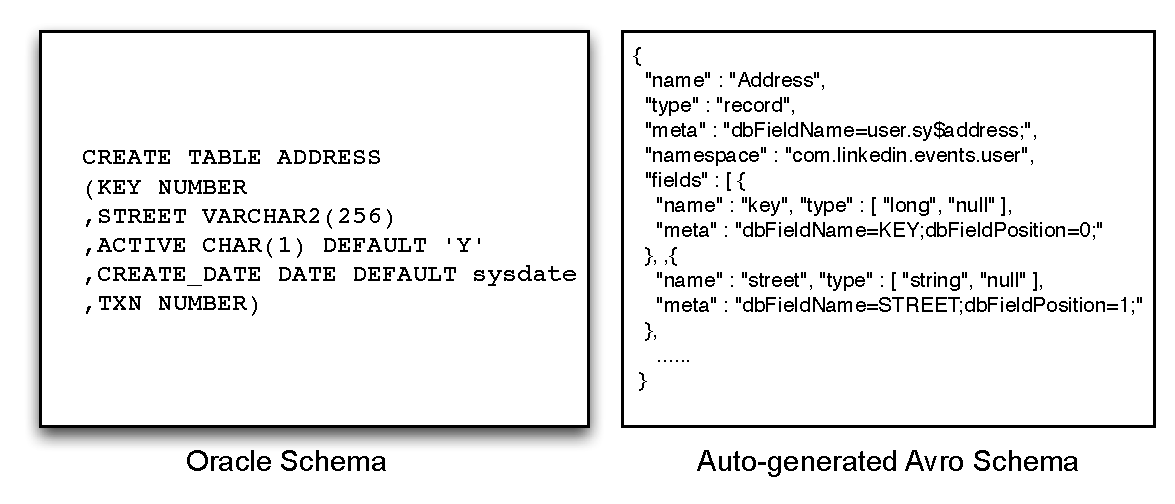
\epsfig{file=figures/oracle-avro-schema.eps, scale=0.75}
\caption{Oracle table mapped to Avro schema}
\label{fig:schema-mapping}
\end{figure*}

Databus uses Avro for serialization of events and supports schema versioning and evolution. This provides an isolation layer that protects consumers from upstream changes in the schema.

The fetchers infer the Avro schema by inspecting the source tables. Figure~\ref{fig:schema-mapping} shows a simple Oracle table mapped to an Avro schema. There are some intricacies when mapping data-types, e.g. when you have a column defined as NUMBER in Oracle, which one of int, long, float do you use when referring to the column in Avro? Once a schema is inferred, the relay is notified about it. When the fetcher generates new events from this table, it serializes the events with the Avro schema. When a table evolves, the schema for it changes and Databus attaches a newer version identifier to it. All new events are now serialized with this new schema version identifier. 

Databus ensures that changes to the source schema do not affect consumers and they can upgrade at their own cadence. The Databus client library performs automatic schema conversion using the standard  Avro schema resolution rules~\cite{avro} . We do not require reserialization of all older events generated since the beginning of time when the schema evolves because all versions of the schema are kept around forever. The schema resolution to an older version of the event schema is performed dynamically at the callback to the consumer. 
